\chapter{Image, Kernel, Rank, and Rank-Nullity}
\label{ch:image-kernel-rank-nullity}

\section*{Chapter Preview}
\addcontentsline{toc}{section}{Chapter Preview}

A linear map may keep some information and erase some information. The image
is the subspace of outputs the map can produce. The kernel is the subspace of
inputs that are erased. Rank-nullity says these two pieces balance exactly.

\section{Image and Kernel}

Let $A\in\R^{m\times n}$, and let $T_A:\R^n\to\R^m$ be the linear map
$T_A(x)=Ax$.

\begin{definition}
The \emph{image} of $A$ is
\[
  \Img A=\{Ax:x\in\R^n\}\subseteq \R^m.
\]
It is the span of the columns of $A$.
\end{definition}

\begin{definition}
The \emph{kernel} of $A$ is
\[
  \Ker A=\{x\in\R^n:Ax=0\}\subseteq \R^n.
\]
\end{definition}

\begin{proposition}
$\Img A$ is a subspace of $\R^m$, and $\Ker A$ is a subspace of $\R^n$.
\end{proposition}

\begin{proof}
If $y_1=Ax_1$ and $y_2=Ax_2$, then
\[
  \lambda y_1+\mu y_2
  =
  A(\lambda x_1+\mu x_2),
\]
so $\Img A$ is closed under linear combinations. If $x_1,x_2\in\Ker A$, then
\[
  A(\lambda x_1+\mu x_2)=\lambda Ax_1+\mu Ax_2=0,
\]
so $\Ker A$ is also closed under linear combinations.
\end{proof}

\section{Kernel as Relations Among Columns}

Write the columns of $A$ as $a_1,\ldots,a_n$. Then
\[
  Ax=x_1a_1+\cdots+x_na_n.
\]
Thus $x\in\Ker A$ exactly when the coefficients in $x$ give a linear relation
among the columns:
\[
  x_1a_1+\cdots+x_na_n=0.
\]

\begin{example}
For
\[
  A=\mat{1&2&3\\2&4&6},
\]
the columns satisfy $-a_1-a_2+a_3=0$. Therefore
\[
  \mat{-1\\-1\\1}\in\Ker A.
\]
\end{example}

\section{Rank and Nullity}

\begin{definition}
The \emph{rank} of $A$ is
\[
  \Rank A=\dim \Img A.
\]
The \emph{nullity} of $A$ is
\[
  \Nullity A=\dim \Ker A.
\]
\end{definition}

Rank is output dimension: how many independent directions the map can produce.
Nullity is lost input dimension: how many independent directions the map sends
to zero.

\begin{figure}[h]
  \centering
  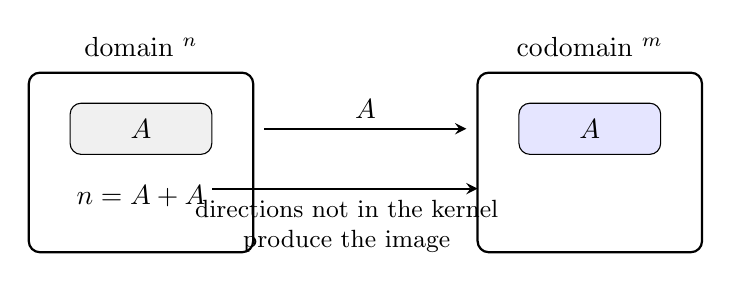
\begin{tikzpicture}[>=stealth,scale=0.95]
    \draw[rounded corners,thick] (-3,-1.2) rectangle (0,1.2);
    \draw[rounded corners,thick] (3,-1.2) rectangle (6,1.2);
    \node at (-1.5,1.55) {domain $\R^n$};
    \node at (4.5,1.55) {codomain $\R^m$};
    \node[draw,fill=gray!12,rounded corners,minimum width=1.8cm,minimum height=0.65cm] at (-1.5,0.45) {$\Ker A$};
    \node[draw,fill=blue!10,rounded corners,minimum width=1.8cm,minimum height=0.65cm] at (4.5,0.45) {$\Img A$};
    \node at (-1.5,-0.45) {$n=\Rank A+\Nullity A$};
    \draw[->,thick] (0.15,0.45) -- node[above] {$A$} (2.85,0.45);
    \draw[->,thick] (-0.55,-0.35) -- (3.0,-0.35);
    \node[align=center,font=\small] at (1.25,-0.85) {directions not in the kernel\\produce the image};
  \end{tikzpicture}
  \caption{Rank-nullity splits the input dimension into erased directions and productive directions.}
\end{figure}

\section{The Rank-Nullity Theorem}

\begin{theorem}[Rank-nullity]
If $A:\R^n\to\R^m$ is linear, then
\[
  \Rank A+\Nullity A=n.
\]
\end{theorem}

\begin{proof}
Let $k_1,\ldots,k_s$ be a basis of $\Ker A$. Extend this list to a basis
\[
  k_1,\ldots,k_s,v_1,\ldots,v_r
\]
of $\R^n$. We claim that $Av_1,\ldots,Av_r$ is a basis of $\Img A$.

It spans $\Img A$: if $y=Ax$, write
\[
  x=\sum_i \alpha_i k_i+\sum_j \beta_j v_j.
\]
Applying $A$ gives
\[
  y=Ax=\sum_j \beta_j Av_j,
\]
because $Ak_i=0$.

It is independent: if $\sum_j \beta_j Av_j=0$, then
\[
  A\left(\sum_j \beta_j v_j\right)=0,
\]
so $\sum_j\beta_jv_j\in\Ker A$. But the full list
$k_1,\ldots,k_s,v_1,\ldots,v_r$ is independent, so all $\beta_j=0$.
Thus $\dim\Img A=r$ and $\dim\Ker A=s$, while $n=r+s$.
\end{proof}

\section{Numerical Rank}

In exact arithmetic, rank is a theorem-level object. On a computer, rank is a
numerical decision. Very small singular values may be mathematical zeros,
rounding noise, or meaningful tiny directions. Lab 3 uses the Hilbert matrix
to show that a theoretically invertible matrix can look rank-deficient in
floating point arithmetic.

\begin{lstlisting}
import numpy as np

A = np.array([[1., 2., 3.],
              [2., 4., 6.]])

rank = np.linalg.matrix_rank(A)
nullity = A.shape[1] - rank

print(rank, nullity, rank + nullity)
\end{lstlisting}

\section*{Chapter Summary}
\addcontentsline{toc}{section}{Chapter Summary}

\begin{itemize}
  \item $\Img A$ is the set of outputs $Ax$ and equals the column span.
  \item $\Ker A$ is the set of inputs sent to zero.
  \item Kernel vectors are linear relations among the columns.
  \item $\Rank A+\Nullity A=n$ for $A:\R^n\to\R^m$.
  \item Numerical rank depends on tolerance and conditioning.
\end{itemize}

\section*{Where This Appears Later}
\addcontentsline{toc}{section}{Where This Appears Later}

Solving $Ax=b$ depends on whether $b\in\Img A$. Least squares projects onto
$\Img A$. The SVD gives orthonormal bases adapted to image, kernel, row space,
and left null space.

\begin{labbox}
Lab 3 implements image/kernel routines, compares exact and floating-point rank,
and uses the Hilbert matrix to expose conditioning.
\end{labbox}

\input{book/exercises/ch05-exercises}
